\chapter{Non-Relativistic Solution of the Hydrogen Molecular Ion in 2 Spatial Dimensions}

\subsection{Existing solutions}

We apply the method used in the 3D case of the $ H_2^{+} $ ion to find the solution in 2 dimensions. The problem itself is analogous to the 3D problem, but leads to the Mathieu's function like solution for the radial problem.

TODO: Add more references
In adition to the Bates paper \cite{Bates1}, there are other, more recent papers \cite{H2Plus2d1} \cite{TwoCentersParticle}, \cite{Kolos} which deal with the solution of the Scrhoedinger equation and spectrum of the $ H_2^{+} $ molecule. TODO: Add more citations.  The solution in \cite{H2Plus2d1} agrees well with our solution There are other solutions, but they rely on the approximative methods, and should be considered inferior to the analytical solution, we provide here. 

Following the 3D case, we rely on Born-Oppenheimer (BO) approximation, in order to provide an analytical solution. The usual justification for using the BO approximation in molecular systems applies to the 2D problems as well, since the masses of the nuclei and electron(s) remain unchanged.  Following the same BO approximation as in Chapter 1, and using atomic units, the Schrodinger equation for the $ H_2^{+} $ molecules is given by equation \eqref{eqPartial2D} below. 

\begin{equation}\label{eqPartial2D}
\left(-\frac{1}{2}\nabla^2-\frac{1}{r_a}-\frac{1}{r_b}\right)\psi = E\,\psi
\end{equation}

The equation \eqref{eqPartial2D} is superficially similar to the equation \eqref{eqPartial3D} and the diagram \ref{h2ion3d}, but in this case, the $ r_a $ and $ r_b $ are vectors in 2 dimensions.

The electron wavefunction depends on only 3 quantum numbers, principal quantum number $ n $, angular quantum number $ l $ and spin $ s $. Again we ignore the spin degrees of freedom,considering the electron to be the regular 3 dimensional particles, where only its orbit is restricted to 2 dimensions.  Therefore the spin magnetic moment of the electron is not affected by the 2D restriction and the spin vector can point in any direction in 3D space. Also the orbit can have different shapes, thus there remains the need for an orbital quantum number. However, there can be one one orientation of the orbit, thus we do not consider the magnetic quantum number. This reasoning agrees with ~The solution of the electron wavefunction to the hydrogen atom in 2 dimensions \cite{H2atom} where electron wavefunction solution only depends on the principal and orbital quantum numbers.

The geometry of the 2D problem leads to choosing the elliptical coordinates (as in 3D problem), with two coordinates, $ \mu $ and $ \lambda $ denoting the position of the electron in 2D plane. \cite{Arfken}

TODO: Add references and more text

\subsection{Exact solution of the  $ H_2^{+} $ electronic Hamiltonian}

The goal is to provide the exact solution to the wavefunction of the $ H_2^{+} $ electron, for a given definition of exact. However even for this, relatively simple problem, it is impossible to find a closed form solution. So the solution is exact, in a sense that it can be done to an arbitrary precision.

\begin{figure}
  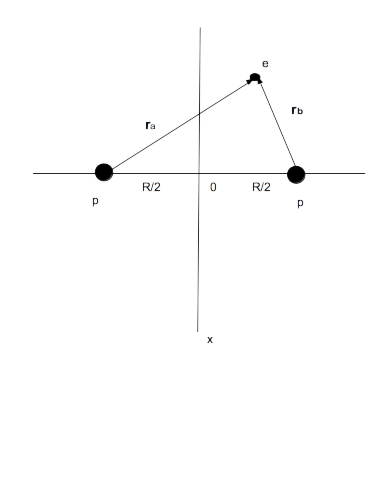
\includegraphics{H2Ion2D.png}
  \caption{H2 Ion in 2D} \label{h2ion2d}
\end{figure}

As illustrated by the figure \ref{h2ion2d}, we express equation \eqref{eqPartial2D} in the elliptical coordinates, and by setting the $ x $ axis to be perpendicular to the internuclear axis, we have the nuclei at: $ y = \pm \frac{R}{2}  $, R being the distance between nuclei. So in  2D elliptic coordinates, $ \lambda $, $ \mu $ we have 
\begin{equation}\label{variables1}
\begin{split}
& \lambda = \left(r_a + r_b\right)/R;\,\,\,\,\,\,\,\,\,\,\,\,\,\,\,\,\,\,\mu =  \left(r_a - r_b\right)/R  \\[1em]
& \text{where } \lambda \in \left[1,\infty\right]\,,\,\,\,\,\,\,\,\,\,\mu \in \left[ -1, 1 \right]\,\,\,\,\,\,\,\,\,\text{ and } \\[.8em] 
& r_a = \frac{R}{2}\left(\lambda + \mu \right)\,\,\,\,\,\,\,\,\,\,\,\,\,\,\,\,\,\,\,\,\,\, r_b = \frac{R}{2}\left(\lambda - \mu \right)
\end{split}
\end{equation}

We assume that the total electronic wavefunction can be written as the product of two functions:
\begin{equation}\label{variables2}
\begin{split}
& \psi(\lambda,\mu) = F(\mu)G(\lambda)
\end{split}
\end{equation}

This way the original equation separates into two ODEs:

\begin{equation}\label{L2-1}
\left(\lambda^2 - 1 \right) \frac{d^2}{ d\lambda^2 }G(\lambda) + \lambda\frac{ d}{d\lambda }G (\lambda)  + \left(A + \frac{E\,R^2}{2}\lambda^2 + 2R\lambda  \right)G (\lambda) = 0  
\end{equation}

\begin{equation}
 \left(1 - \mu^2 \right) \frac{d^2}{ d\mu^2 }F(\mu) - \mu\frac{ d }{d\mu }F(\mu) +  \left(-A -  \frac{E\,R^2}{2}\mu^2  \right)F(\mu) = 0
\end{equation}
where
\begin{equation}\label{eqP}
p^2 = -\frac{E\,R^2}{2}
\end{equation}

$ A $ is the separation constant.  To eliminate the singularities, and following \cite{H2Plus2d1} we introduce two new functions:
\begin{equation}\label{eqNew}
\begin{split}
& F(\mu) = (1-\mu^2)^{k/2}M(\mu) \\[.8em]
& G(\lambda) = (\lambda^2-1)^{k/2}L(\lambda)
\end{split}
\end{equation}
to obtain
\begin{equation}
\begin{split}
& \frac{d\,F}{d\mu} =  (1-\mu^2)^{k/2}\frac{d\,M}{d\mu} - k\mu(1-\mu^2)^{k/2-1}M(\mu) \\[.8em]
& \frac{d^2\,F}{d\mu^2} =  (1-\mu^2)^{k/2}\frac{d^2\,M}{d\mu^2} - 21Gk\mu(1-\mu^2)^{k/2-1}\frac{d\,M}{d\mu} + \\[.8em]
& + \left[2\left(\frac{k}{2}-1\right)k\mu^2\left(1-\mu^2\right)^{k/2-2} - k(1 - \mu^2)^{k/2-1}\right]M
\end{split}
\end{equation}

\begin{equation}
\begin{split}
& \frac{d\,G}{d\lambda} =  (\lambda^2-1)^{k/2}\frac{d\,L}{d\lambda} + k\lambda(\lambda^2-1)^{k/2-1}L(\lambda) \\[.8em]
& \frac{d^2\,G}{d\lambda^2} =  (\lambda^2-1)^{k/2}\frac{d^2\,L}{d\lambda^2} + 2k\lambda(\lambda^2-1)^{k/2-1}\frac{d\,L}{d\lambda} + \\[.8em]
& + \left[2\left(\frac{k}{2}-1\right)k\mu^2\left(\lambda^2-1\right)^{k/2-2} - k(\lambda^2-1)^{k/2-1}\right]L
\end{split}
\end{equation}
Plug in:
\begin{equation}
\begin{split}
& (1-\mu^2)(1-\mu^2)^{k/2}\frac{d^2\,M}{d\mu^2}  - (1-\mu^2)2k\mu(1-\mu^2)^{k/2-1}\frac{d\,M}{d\mu}  + \\[.8em]
& + (1-\mu^2)\left[2\left(\frac{k}{2}-1\right)k\mu^2\left(1-\mu^2\right)^{k/2-2} - k(1 - \mu^2)^{k/2-1}\right]M - \\[.8em]
& - \mu (1-\mu^2)^{k/2}\frac{d\,M}{d\mu} +  k\mu^2(1-\mu^2)^{k/2-1}M(\mu) + \\[.8em]
& + \left(-A -  \frac{E\,R^2}{2}\mu^2  \right) (1-\mu^2)^{k/2}M(\mu)  = 0
\end{split}
\end{equation}
Or dividing by $ (1-\mu^2)^{k/2} $:
\begin{equation}
\begin{split}
& (1-\mu^2)\frac{d^2\,M}{d\mu^2} - (2k+1)\mu\frac{d\,M}{d\mu} +   \left[ A -  \frac{E\,R^2}{2}\mu^2  + k(k-1)\frac{\mu^2}{1-\mu^2} - k  \right]M = 0
\end{split}
\end{equation}
And for the other equation, plug in:
\begin{equation}
\begin{split}
&  (\lambda^2-1)(\lambda^2-1)^{k/2}\frac{d^2\,L}{d\lambda^2} +  (\lambda^2-1)2k\lambda(\lambda^2-1)^{k/2-1}\frac{d\,L}{d\lambda} + \\[.8em]
& + \left[2\left(\frac{k}{2}-1\right)k\lambda^2\left(\lambda^2-1\right)^{k/2-2} - k(\lambda^2-1)^{k/2-1}\right](\lambda^2-1)L + \\[.8em]
& + \lambda (\lambda^2-1)^{k/2}\frac{d\,L}{d\lambda} + k\lambda^2(\lambda^2-1)^{k/2-1}L(\lambda)  + \\[.8em]
& +  \left(A + \frac{E\,R^2}{2}\lambda^2 + 2R\lambda  \right) (\lambda^2-1)^{k/2}L(\lambda) = 0
\end{split}
\end{equation}
Or dividing by $ (\lambda^2 - 1)^{k/2} $:
\begin{equation}
\begin{split}
& (\lambda^2-1)\frac{d^2\,L}{d\lambda^2} + (2k+1)\lambda \frac{d\,L}{d\lambda} +  \left[A + \frac{E\,R^2}{2}\lambda^2 + 2R\lambda  -k + k(k-1)\frac{\lambda^2}{\lambda^2-1} \right]L = 0
\end{split}
\end{equation}

To make both $ M(\mu) $ and $ L(\lambda) $ non singular at $ \mu, \lambda= 1$ we must have the $ k = 0, 1 $. So the equations reduces to:
\begin{equation}\label{M1}
\begin{split}
& (1-\mu^2)\frac{d^2\,M}{d\mu^2}  - (2k+1)\mu\frac{d\,M}{d\mu} +   \left[ A -  \frac{E\,R^2}{2}\mu^2  -  k  \right]M(\mu) = 0 \\[.8em]
\end{split}
\end{equation}
\begin{equation}\label{L1}
\begin{split}
& (\lambda^2-1)\frac{d^2\,L}{d\lambda^2} + (2k+1)\lambda \frac{d\,L}{d\lambda} +  \left[A + \frac{E\,R^2}{2}\lambda^2 + 2R\lambda  -k \right]L(\lambda) = 0
\end{split}
\end{equation}

Effectively the choice of parameter $ k $ determines the parity of the solution. At this point we set:

\begin{equation}
p^2 = -\frac{ER^2}{2}
\end{equation}

And proceed with solving each equation separately:

\subsubsection{ M Equation }

Using the substition $ \mu = \cos x $ we get the other form of the equation:

\begin{equation}\label{M2}
M^{''}(x) - 2k M^{'}(x) +   \left[ A - k + \frac{p^2}{2} + \frac{p^2}{2}\mu^2\cos(2x)  \right]M(x) = 0
\end{equation}

The equation \eqref{M2} is a form of a angular Mathieu's equation \cite{Mathieu2}, thus we look for the solution in the form of:
\begin{equation}\label{MSol}
\begin{split}
& M(\mu) = \sum_{n=1}^{\infty}{a_n\,e^{i2nx}} \\[.8em]
\end{split}
\end{equation}
The solution depends on the chosen boundary conditions. The angular Mathieu's equation admits an even and odd solution, with respect to the origin. The parity of the solution is chosen depending on the boundary conditions for a particular problem. Therefore

\begin{equation}\label{Meven}
\begin{split}
& \text{ For the even case, the boundary condition is } \\[.8em]
& M(\mu = 1) = M(\mu = -1) = 1\,;\,\,\Rightarrow  M'(0) = M'\left(\frac{\pi}{2}\right) = 0 \Rightarrow \\[.8em] 
& \text{ The solution is then in the form } \\[.8em]
& M(\mu) = \sum_{n=1}^{\infty}{a_n \cos\left(n\,\mu\right)}
\end{split}
\end{equation}

\begin{equation}\label{Modd1}
\begin{split}
& \text{ And for the odd case, take the boundary conditions: } \\[.8em]
& M(\mu = 1) = 1\,;\,\,M(\mu = -1) = -1\,;\,\,\Rightarrow  M(0) = M'\left(\frac{\pi}{2}\right) = 0 \Rightarrow \\[.8em] 
\end{split}
\end{equation}
\begin{equation}\label{Modd2}
\begin{split}
& \text{ The solution is then in the form: } \\[.8em]
& M(\mu) = \sum_{n=1}^{\infty}{a_n \sin\left[\left(2n+1\right)\,\mu\right]} 
\end{split}
\end{equation}

From now on, the solution to the equation for $ M(\mu) $ \eqref{M2} is straightforward. Set the boundary conditions, and express  $ M(\mu) $ in the series of sine or cosine functions.

\subsubsection{ L Equation }

\begin{equation}\label{L2-2}
\begin{split}
& (\lambda^2-1)\frac{d^2\,L}{d\lambda^2} + (2k+1)\lambda \frac{d\,L}{d\lambda} +  \left[A + \frac{E\,R^2}{2}\lambda^2 + 2R\lambda  -k \right]L(\lambda) = 0
\end{split}
\end{equation}

The equation for the $ L(\lambda) $ looks similar to the radial (modified) Mathieu equation, but it is not an exact identity. 

We observe that both equations for the function $ M(\mu) $ and $ L(\lambda) $ are related to the Mathieu's equations. In general the Mathieu's equation represents the standing wave on an elliptical drum, (2D space),  and the solution for the time independent Schroedinger equation is in general a standing wave, in 2D in this case. So it is plausible that these types of slutions are similar.

For the equation \eqref{L2-2} one could proceed by following the radial Mathieu's equations approach. One way to solve the Radial Mathieu's equation is by using the series of hyperbolic functions, obtained from the solution of angular Mathieu's equation using the substitution $ \eta = i\,\xi$.  But that this approach in numerically unstable and hard to compute \cite{Mathieu4}. There is another approach, using the product of Bessel Functions \cite{Mathieu4}

We took a different approach to solving the equation \eqref{L2-2}, namely look for the solution in the form of the series of orthogonal functions. This approach has some challenges, since there are number of functions orthogonal on a finite interval, and one can choose the one which fits the problem the best. On an infinite interval, such as $ \lambda = [1, \infty] $ the choice is somewhat limited. The Laguerre's polynomial seemed like a suitable choice, as they form an orthogonal set on the infinite interval. So we look for the solution in the form:

\begin{equation}\label{Lsol1}
\begin{split}
& L(\lambda) =  e^{-p\lambda}\sum_{n=0}^{\infty}{c_n\,L_n(\lambda)}
\end{split}
\end{equation}

Where $ L_n(\lambda) $ are Laguerre polynomials. They have several interesting properties, which can be found in \cite{Laguerre1}.

\subsubsection{ Towards the solution }

So using the solutions above, the next step is to find the eigenvalues $ A $, $ p $, of the equations \eqref{M1} and \eqref{L2-2} for the values of $ k = 0,1 $. Using the series above, for each equation, we find function  $ A_i(p) $ for which the solution exists. The intersection of the two functions $ A_i(p) $ is the value of $ p $ common for both equations \eqref{M1} \eqref{L2-2}. This procedure translates into the matrix eigenvalues problem, following the steps below.

For the even M equation, we insert the solution \eqref{Meven} in the equation {eqFinal}, multiply by $ \cos(2m\,x) $, $ m = 0,1,2,... $ and integrate. Since the basis functions in the series are orthogonal we obtain:

\begin{equation}
\begin{split}
& \sum_{n=0}^{\infty}c_k \left\{-4n^2\int_{-\pi/2}^{\pi/2}{\cos(2 mx)\cos(2 nx)dx} + \left[ \frac{p^2}{2} +k \right]\int_{-\pi/2}^{\pi/2}{\cos(2 mx)\cos(2 nx)dx} + \right. \\[.8em]
& \left. + \left[ \frac{p^2}{2} + k\right] \int_{-\pi/2}^{\pi/2}{\cos(2 x)\cos(2 mx)\cos(2 nx)dx} \right\} = \\[.8em]
& = A \int_{-\pi/2}^{\pi/2}{\cos(2 mx)\cos(2 nx)dx}  \,\Longrightarrow\\[.8em]
\end{split}
\end{equation}
or
\begin{equation}
\begin{split}
& \frac{p^2}{2}\pi\,\delta_{0,0}  +  \left[ \frac{p^2}{2} +k\right]\frac{\pi}{2}\delta_{0,1} + \left[\frac{p^2}{2} + k\right] \frac{\pi}{2}\delta_{1,0} + \sum_{m=1}^{\infty}\sum_{n=1}^{\infty} {\left(-4n^2 +\frac{p^2}{2}\right)\frac{\pi}{2} \delta_{m,n} } + \\[.8em]
& + \left[\frac{p^2}{2}+k\right]\frac{\pi}{4}\delta_{m,n+1} + \left[\frac{p^2}{2}+k\right]\frac{\pi}{4}\delta_{m,n-1}  = A \pi\,\delta_{0,0} + \sum_{m=1}^{\infty}\sum_{n=1}^{\infty}{A\frac{\pi}{2}\delta_{m,n}}\,\,\,\Longrightarrow \\[.8em]
& p^2\delta_{0,0} +  \left[ \frac{p^2}{2}+k\right]\delta_{0,1} + \left[ \frac{p^2}{2}+k\right]\delta_{1,0} + \sum_{m=1}^{\infty}\sum_{n=1}^{\infty}{\left\{ -4k^2\,\delta_{m,n} + \frac{p^2}{2}\,\delta_{m,n} +  \left[ \frac{p^2}{4} +k \right]\,\delta_{m,n \pm 1} \right\}} = \\[.8em]
& = 2\,A+ \sum_{m=1}^{\infty}\sum_{n=1}^{\infty}{A\,\delta_{m,n}}
\end{split}
\end{equation}\\*

For the odd case, inseert the equation \eqref{Modd2} in the equation {eqFinal}, multiply by $ \sin[(2m+1)\,x] $, $ m = 0,1,2,3... $ and integrate (again exploiting the orthogonality of the basis functions):
\begin{equation}
\begin{split}
& \sum_{n=0}^{\infty}c_k -(2n+1)^2\int_{-\pi/2}^{\pi/2}{\sin[(2 m+1)x]\sin[(2 n+1)x]dx} + \left[\frac{p^2}{2} + k \right]\int_{-\pi/2}^{\pi/2}{\sin[(2 m+1)x]\sin[(2 n+1)x]dx} +  \\[.8em]
& + \left[ \frac{p^2}{2} +k \right] \int_{-\pi/2}^{\pi/2}{\cos(2 x)\sin[(2 m+1)x]\sin[(2 k+1)x]dx}   = A \int_{-\pi/2}^{\pi/2}{\sin[(2 m+1)x]\sin[(2 k+1)x]dx}  \Longrightarrow \\[.8em]
\end{split}
\end{equation}\\*
\begin{equation}
\begin{split}
&  \left[ - \frac{\pi}{2} + \frac{\pi}{2}\frac{p^2}{2} - \frac{\pi}{4}\frac{p^2}{2}\right]\delta_{0,0} +  \frac{\pi}{4}\left[\frac{p^2}{2}+k\right]\delta_{0,1} + \left[\frac{\pi}{4}+ k\right]\frac{p^2}{2}\delta_{1,0}  + \\[.8em]
& +  \sum_{m=1}^{\infty}\sum_{n=1}^{\infty} {\left[-(2n+1)^2 + \frac{p^2}{2}\right] \frac{\pi}{2}\delta_{m,n} +  \left[\frac{p^2}{2}+k\right]\frac{\pi}{4}\delta_{m,n \pm 1} } = \\[.8em]
&  = A\frac{\pi}{2}\delta_{0,0}  + A\frac{\pi}{2}  \sum_{m=1}^{\infty}\sum_{n=1}^{\infty} {\delta_{m,n}} \Longrightarrow
\\[.8em]
\end{split}
\end{equation}\\*
\begin{equation}
\begin{split}
& \left( - 1 + \frac{p^2}{4} \right)\delta_{0,0} + \left[ \frac{p^2}{4} + k \right]\delta_{0,1}  + \left[ \frac{p^2}{4} +k \right]\delta_{1,0}  + \\[.8em]
& + \sum_{m=1}^{\infty}\sum_{n=1}^{\infty} {\left(-(2n+1)^2 + \frac{p^2}{2}\right) \delta_{m,n} +  \left[\frac{p^2}{4}+k\right]\delta_{m,n \pm 1} } = \\[.8em]
&  = A\delta_{0,0}  + A  \sum_{m=1}^{\infty}\sum_{n=1}^{\infty} {\delta_{m,n}}
\end{split}
\end{equation}\\*

For the $ L $ equation, first by shifting the origin $ x = \lambda -1 $ and by using various properties of Laguerre polynomials and its derivatives \cite{Laguerre1} we obtain.

\begin{equation}
\begin{split}
&  \sum_{n=0}^{\infty}c_n \left\{ \sum_{i = 0}^{n-1}{L_i(x)}  +  \right. \\[.8em] 
& + \left[ -2pn(2n+1) -(2p-1)n^2 -4pn +(2R-p)(2n+1) - p^2 -p + 2R \right]L_n + \\[.8em]
& + \left[2pn(n+1) - (2R-p)(n+1) \right]L_{n+1} + \\[.8em]
& + \left[2pn^2 + (2p-1)n(2n-1) + (4p-2)n - (2R-p)n \right]L_{n-1} - \\[.8em]
& \left. - \left[ (2p-1)n(n-1)  \right]L_{n-2}  \right\}
\end{split}
\end{equation}\\[1em]

Now multiply by $ L_m(x) $ and use the orthogonality of Laguerre's polynomials. 

\begin{equation}
\begin{split}
& \int_0^{\infty} \sum_{n=0}^{\infty}c_n \sum_{m=0}^{\infty}L_m(x) \left\{ \sum_{i = 0}^{n-1}{L_i(x)}  +  \right. \\[.8em] 
& + \left[ -2pn(2n+1) -(2p-1)n^2 -4pn +(2R-p)(2n+1) - p^2 -p + 2R \right]L_n + \\[.8em]
& + \left[2pn(n+1) - (2R-p)(n+1) \right]L_{n+1} + \\[.8em]
& + \left[2pn^2 + (2p-1)n(2n-1) + (4p-2)n - (2R-p)n \right]L_{n-1} - \\[.8em]
& \left. - \left[ (2p-1)n(n-1)  \right]L_{n-2}  \right\}
\end{split}
\end{equation}\\[1em]

The result is an "almost" lower triangular matrix, called Hessenberg matrix.

The rest of the work is numerical. Since our goal is to obtain the function $ E(R) $ we choose the suitable values of $ R $ as in table \ref{groundEven} . For each value of $ R $ we divide with the interval $ p \in [0,2*R] $ into the $ n $ points. For each value of $ p $ we calculate store the eigenvalues for equation for $ M(\mu) $ and $ L(\lambda) $. Finding matrix eigenvalues is a common operation is a number of fields, and good numerical algorithms and libraries are available, such as \cite{Lapack1}.  Regardless, finding eigenvalues is a relative slow operation, with the complexity $ O(n^\omega), 2 < \omega \le 3 $, \cite{Lapack1} $ n $ being the size of the matrix.  Eigenvalues for matrices up to $ 100 \times 100 $, i.e. limiting the sums above to 100 elements can be found using Wolfram Mathematica, within a reasonable time. However for $ n \ge 100 $ the time needed increases as $ n^3 $ \cite{QRDecomposition1} \cite{LinearAlgebra1} and the Mathematica becomes unusable. For $  n = 1000 $, i.e $ 1000 \times 1000  $ matrices I used the Fortran Gnu compiler and Lapack \cite{Lapack1} libraries. The Lapack libraries are both accurate and fast, and it took about 30 minutes to find an eigenvalue on Apple Macbook Pro, with 16GB ram and Intel I7 processor at 2.2 GHz.

In comparison, the results obtain by using Wolfram Mathematica for $ n = 100 $ and results using Lapack for $ n = 1000 $  agree up to one part in $ 10^{-3} $.

Once the eigenvalues are calculated we have two functions $ A_i(p) $ for each of the equations. Interpolate and find the value of $ p $ for which the curves intersect. From the value of $ p $ we obtain the eigenenergy $ E = E(R) $ using equation \eqref{eqP}.

TODO: Check stability, i.e obtain a and q from A and p.

\subsection{Plots, Tables, etc... }

Table depicting the calculated energies of the electron for the ground state (even and odd) and first and second excited state: (TODO: wording, captions ) . Also TODO: note that it does not work for small R (needs more points). All numbers are in atomic units.

\afterpage{
  \newgeometry{left=4em,right=3em,top=5em,bottom=5em}
  \captionof{table}{Ground State, Even Energies} 
  \label{groundEven}
  \rotatebox{90}{
		\begin{tabular}{ >{\bfseries}m{4em} m{4em}  m{4em}  m{4em} }
			\hline
			R & p & A & E \\ \hline \hline
			.2 & -1 & -1 & -1 \\[-1em]
			.4 & 0.6482991 & 0.215659 & -5.2536 \\[-1em]
			.6 & 0.8968546 & 0.422304 & -4.4686  \\[-1em]
			.8 & 1.1214876 & 0.677779 & -3.93042 \\[-1em]
			1.0 & 1.3311023 & 0.982007 & -3.54367 \\[-1em]
			1.2 & 1.5312058 & 1.33809 & -3.25638 \\[-1em]
			1.4 & 1.7254930 & 1.75074 & -3.03809 \\[-1em]
			1.6 & 1.9165547 & 2.22543 & -2.86967 \\[-1em]
			1.8 & 2.1062223 & 2.76777 & -2.73838 \\[-1em]
			2.0 & 2.2957553 & 3.38297 & -2.63525 \\[-1em]
			2.2 & 2.4859626 & 4.07548 & -2.55372 \\[-1em]
			2.4 & 2.6772997 & 4.84875 & -2.48887 \\[-1em]
			2.6 & 2.8699576 & 5.70516 & -2.4368 \\[-1em]
			2.8 & 3.0639450 & 6.64611 & -2.39484 \\[-1em]
			3.0 & 3.2591587 & 7.67222 & -2.36047 \\[-1em]
			3.2 & 3.4554388 & 8.78351 & -2.33204 \\[-1em]
			3.4 & 3.6526076 & 9.97968 & -2.30823 \\[-1em]
			3.6 & 3.8504933 & 11.2602 & -2.28801 \\[-1em]  
			3.8 & 4.0489429 & 12.6244 & -2.27063 \\[-1em]
			4.0 & 4.2478273 & 14.0717 & -2.2555 \\[-1em]
			4.2 & 4.4470414 & 15.6016 & -2.2422 \\[-1em]
			4.4 & 4.6465020 & 17.2136 & -2.23037 \\[-1em]
			4.6 & 4.8461448 & 18.9072 & -2.21977 \\[-1em]
			4.8 & 5.0459206 & 20.6821 & -2.21018 \\[-1em]
			5.0 & 5.2457926 & 22.5380 & -2.20147 \\[-1em]
			5.5 & 5.7457302 & 27.5309 &  -2.18271 \\[-1em]
			6.0 & 6.2458515 & 33.0265 & -2.16726 \\[-1em]
			6.5 & 6.7460376 & 39.0236 & -2.15427 \\[-1em]
			7.0 & 7.2462380 & 45.5215 & -2.14318  \\[-1em]
			7.5 & 7.7464325 & 52.5198 & -2.13359 \\[-1em]
			8.0 & 8.2466140 & 60.0184 & 2.12521 \\[-1em]
			8.5 & 8.7467810 & 68.0173 & -2.11782 \\[-1em]
			9.0 & 9.2469337 & 76.5162 & -2.11125 \\
			\hline
		\end{tabular}
	}
	\\[4.em]
	\rotatebox{90}{
		\begin{tabular}{ m{4em} m{4em}  m{4em}  m{4em} }
			\hline
			R & p & A & E \\ \hline \hline
			9.5 & 9.7470735 & 85.5153 & -2.10538 \\[-1em]
			10.0 & 10.247201 & 95.0145 & -2.1001  \\[-1em]
			10.5 & 10.747319 & 105.014 & -2.09533  \\[-1em]
			11.0 & 11.247427 & 115.513 & -2.09099  \\[-1em]
			11.5 & 11.747527 & 126.513 & -2.08702  \\[-1em]
			12.0 & 12.247620 & 138.012 & -2.08339  \\[-1em]
			12.5 & 12.747706 & 150.012 & -2.08005  \\[-1em]
			13.0 & 13.247787 & 162.511 & -2.07697  \\[-1em]
			13.5 & 13.747862 & 175.511 & -2.07411  \\[-1em]
			14.0 & 14.247932 & 189.010 & -2.07147  \\[-1em]
			14.5 & 14.747997 & 203.010 & -2.06899  \\[-1em]
			15.0 & 15.248059 & 217.510 & -2.06669  \\[-1em]
			15.5 & 15.748117 & 232.509 & -2.06454 \\[-1em]
			16.0 & 16.248172 & 248.009 & -2.06252 \\[-1em]
			16.5 & 16.748223 & 264.009 & -2.06063 \\[-1em]
			17.0 & 17.248272 & 280.508 & -2.05884 \\[-1em]
			17.5 & 17.748318 & 297.508 & -2.05716 \\[-1em]
			18.0 & 18.248362 & 315.008 & -2.05557 \\[-1em]
			18.5 & 18.748404 & 333.008 & -2.05407 \\[-1em]
			19.0 & 19.248443 & 351.508 & -2.05265 \\[-1em]
			19.5 & 19.748481 & 370.507 &  -2.05129 \\[-1em]
			20.0 & 20.248517 & 390.007 &  -2.05001 \\[-1em]
			20.5 & 20.748551 & 410.007 &  -2.04879 \\[-1em]
			21.0 & 21.248584 & 430.507 &  -2.04763 \\[-1em]
			21.5 & 21.748615 & 451.507 &  -2.04652 \\[-1em]
			22.0 & 22.248645 & 473.006 &  -2.04546 \\[-1em]
			22.5 & 22.748673 & 495.006 &  -2.04445 \\[-1em]
			23.0 & 23.248701 & 517.506 &  -2.04349 \\[-1em]
			23.5 & 23.748727 & 540.506 &  -2.04256 \\[-1em]
			24.0 & 24.248753 & 564.006 &  -2.04167 \\[-1em]
			24.5 & 24.748777 & 588.006 &  -2.04082 \\[-1em]
			25.0 & 25.248800 & 612.506 &   -2.04001 \\
			\hline
		\end{tabular}
	}
	\restoregeometry
}

\afterpage{
  \newgeometry{left=4em,right=3em,top=5em,bottom=5em}
  \captionof{table}{Ground State, Odd Energies} \label{tab:groundOdd}
  \rotatebox{90}{
		\begin{tabular}{ m{4em} m{4em}  m{4em}  m{4em} }
		\hline
		    R & p & A & E \\ \hline \hline
        0.2 & 0.2002000 & -0.989967 & -2.004 \\[-1em]
        0.4 & 0.2899422 & -0.978928 & -1.05083 \\[-1em]
        0.6 & 0.4698674 & -0.944425 & -1.22653 \\[-1em]
        0.8 & 0.6583497 & -0.890176 & -1.35445 \\[-1em]
        1. & 0.83893725 & -0.820177 & -1.40763 \\[-1em]
        1.2 & 1.0072282 & -0.738337 & -1.40904 \\[-1em]
        1.4 & 1.1637570 & -0.647105 & -1.38197 \\[-1em]
        1.6 & 1.3101216 & -0.547923 & -1.34095 \\[-1em]
        1.8 & 1.4478995 & -0.441659 & -1.29408 \\[-1em]
        2. & 1.57842277 & -0.328846 & -1.24571  \\[-1em]
        2.2 & 1.7027722 & -0.209819 & -1.19811  \\[-1em]
        2.4 & 1.8218201 & -0.084788 & -1.15244 \\[-1em]
        2.6 & 1.9362735 & 0.0461182 & -1.10922  \\[-1em]
        2.8 & 2.0467105 & 0.182823 & -1.06863  \\[-1em]
        3. & 2.15360935 & 0.325285 & -1.03067 \\[-1em]
        3.2 & 2.2573686 & 0.473487 & -0.995256  \\[-1em]
        3.4 & 2.3583242 & 0.627428 & -0.962231  \\[-1em]
        3.6 & 2.4567615 & 0.787117 & -0.931432  \\[-1em]
        3.8 & 2.5529247 & 0.952568 & -0.90269  \\[-1em]
        4. & 2.64702425 & 1.1238 & -0.875842 \\[-1em]
        4.2 & 2.7392425 & 1.30082 & -0.850731 \\[-1em]
        4.4 & 2.8297387 & 1.48366 & -0.827213 \\[-1em]
        4.6 & 2.9186522 & 1.67232 & -0.805154 \\[-1em]
        4.8 & 3.0061054 & 1.86681 & -0.784433 \\[-1em]
        5. & 3.09220669 & 2.06715 & -0.764939 \\[-1em]
        5.5 & 3.3021488 & 2.59351 & -0.720938 \\[-1em]
        6. & 3.50544693 & 3.15618 & -0.682675 \\[-1em]
        6.5 & 3.7030358 & 3.75479 & -0.649111 \\[-1em]
        7. & 3.89563406 & 4.38877 & -0.619427 \\[-1em]
        7.5 & 4.0838013 & 5.05737 & -0.592975 \\[-1em]
        8. & 4.26798013 & 5.7597 & -0.569239 \\[-1em]
        8.5 & 4.4485253 & 6.49477 & -0.547803 \\[-1em]
        9.0 & 4.62572636 & 7.26153 & -0.528329 \\
		\hline
		\end{tabular}
    }
    \\[4.em]
    \rotatebox{90}{
		\begin{tabular}{ m{4em} m{4em}  m{4em}  m{4em} }
		\hline
		    R & p & A & E \\ \hline \hline
        9.5 & 4.7998226 & 8.05888 & -0.510544 \\[-1em]
        10.0 & 4.971016 & 8.88573 & -0.49422 \\[-1em]
        10.5 & 5.139479 & 9.74099 & -0.47917 \\[-1em]
        11.0 & 5.305363 & 10.6236 & -0.465238 \\[-1em]
        11.5 & 5.468800 & 11.5325 & -0.452292 \\[-1em]
        12.0 & 5.629908 & 12.4667 & -0.44022 \\[-1em]
        12.5 & 5.788793 & 13.4253 & -0.42893 \\[-1em]
        13.0 & 5.945554 & 14.4073 & -0.418339 \\[-1em]
        13.5 & 6.100278 & -0.40837 & -0.408378 \\[-1em]
        14.0 & 6.253049 & 16.4385 & -0.398986 \\[-1em]
        14.5 & 6.403943 & 17.4861 & -0.39011 \\[-1em]
        15.0 & 6.553030 & 18.554 & -0.381709 \\[-1em]
        15.5 & 6.700378 & 19.6416 & -0.373736 \\[-1em]
        16.0 & 6.846048 & 20.7482 & -0.366159 \\[-1em]
        16.5 & 6.990098 & 21.8732 & -0.358946 \\[-1em]
        17.0 & 7.132585 & 23.016 & -0.352068 \\[-1em]
        17.5 & 7.273559 & 24.1762 & -0.3455 \\[-1em]
        18.0 & 7.413071 & 25.3531 & -0.33922 \\[-1em]
        18.5 & 7.551165 & 26.5464 & -0.333207 \\[-1em]
        19.0 & 7.687887 & 27.7555 & -0.327444 \\[-1em]
        19.5 & 7.823278 & 28.98 & -0.321913 \\[-1em]
        20.0 & 7.957378 & 30.2195 & -0.316599 \\[-1em]
        20.5 & 8.090224 & 31.4735 & -0.311489 \\[-1em]
        21.0 & 8.221852 & 32.7418 & -0.306571 \\[-1em]
        21.5 & 8.352296 & 34.0239 & -0.301832 \\[-1em]
        22.0 & 8.481589 & 35.3195 & -0.297262 \\[-1em]
        22.5 & 8.609763 & 36.6282 & -0.292851 \\[-1em]
        23.0 & 8.736845 & 37.9498 & -0.288592 \\[-1em]
        23.5 & 8.862866 & 39.2839 & -0.284474 \\[-1em]
        24.0 & 8.987851 & 40.6303 & -0.280491 \\[-1em]
        24.5 & 9.111828 & 41.9886 & -0.276636 \\[-1em]
        25.0 & 9.234820 & 43.3586 & -0.272902 \\
		\hline
		\end{tabular}
	}
	\restoregeometry
}

\afterpage{
  \newgeometry{left=4em,right=3em,top=5em,bottom=5em}
  \captionof{table}{First Excited State, Even Energies} \label{tab:firstEven}
  \rotatebox{90}{
		\begin{tabular}{ m{4em} m{4em}  m{4em}  m{4em} }
		\hline
		    R & p & A & E \\ \hline \hline
		\hline
		\end{tabular}
    }
    \\[4.em]
    \rotatebox{90}{
		\begin{tabular}{ m{4em} m{4em}  m{4em}  m{4em} }
		\hline
		    R & p & A & E \\ \hline \hline
		\hline
		\end{tabular}
	}
	\restoregeometry
}

\afterpage{
  \newgeometry{left=4em,right=3em,top=5em,bottom=5em}
  \captionof{table}{First Excited State, Odd Energies} \label{tab:firstOdd}
  \rotatebox{90}{
		\begin{tabular}{ m{4em} m{4em}  m{4em}  m{4em} }
		\hline
		    R & p & A & E \\ \hline \hline
		\hline
		\end{tabular}
    }
    \\[4.em]
    \rotatebox{90}{
		\begin{tabular}{ m{4em} m{4em}  m{4em}  m{4em} }
		\hline
		    R & p & A & E \\ \hline \hline
		\hline
		\end{tabular}
	}
	\restoregeometry
}

\afterpage{
  \newgeometry{left=4em,right=3em,top=5em,bottom=5em}
  \captionof{table}{Second Excited State, Even Energies} \label{tab:secondEven}
  \rotatebox{90}{
		\begin{tabular}{ m{4em} m{4em}  m{4em}  m{4em} }
		\hline
		    R & p & A & E \\ \hline \hline
		\hline
		\end{tabular}
    }
    \\[4.em]
    \rotatebox{90}{
		\begin{tabular}{ m{4em} m{4em}  m{4em}  m{4em} }
		\hline
		    R & p & A & E \\ \hline \hline
		\hline
		\end{tabular}
	}
	\restoregeometry
}

\afterpage{
  \newgeometry{left=4em,right=3em,top=5em,bottom=5em}
  \captionof{table}{Second Excited State, Odd Energies} \label{tab:secondOdd}
  \rotatebox{90}{
		\begin{tabular}{ m{4em} m{4em}  m{4em}  m{4em} }
		\hline
		    R & p & A & E \\ \hline \hline
		\hline
		\end{tabular}
    }
    \\[4.em]
    \rotatebox{90}{
		\begin{tabular}{ m{4em} m{4em}  m{4em}  m{4em} }
		\hline
		    R & p & A & E \\ \hline \hline
		\hline
		\end{tabular}
	}
	\restoregeometry
}
